\documentclass[10pt]{article}
\usepackage[margin=1in]{geometry}
\usepackage{amsmath,booktabs,graphicx,hyperref}
\hypersetup{hidelinks}
\title{Beyond Relevance: Dependency-Aware and Temporally Grounded Evidence Verification for Reliable Generative Search}
\author{Rahul Chaube\\Independent VERITAS project}
\date{Technical report, 24 November 2026}
\begin{document}
\maketitle
\begin{abstract}
Search results can count the same report many times. We investigate a local claim verifier that groups potentially dependent documents, excludes temporally ineligible evidence, and caps each group's contribution to each stance. On a controlled experiment with one supporting and one opposing observation, duplicating the opposing report up to sixteen times left the signed evidence balance unchanged when both observations remained visible. Under a ten-document budget, duplicates could crowd the primary source out of the candidate set. On SciFact, BM25 retrieved gold abstracts more effectively than our lightweight rank fusion. On an 80-claim neural comparison, a learned passage filter gave 18 decisive answers, of which 11 matched gold verdicts. Six of 19 citations matched annotated rationales. These findings isolate a property of aggregation while exposing substantial uncertainty in the evidence used by the verifier.
\end{abstract}
\section{Question and prior work}
When does a collection of retrieved pages supply multiple observations about a claim? Source-dependent truth discovery already models copying, and Knowledge-Based Trust estimates reliability from extracted facts \cite{Dependence,KBT}. Recent work evaluates conflicting sources and temporally changing evidence \cite{CONFACT,FreshLLMs,LiveFact}. SAFE checks atomic propositions using search, and ALCE evaluates citation quality \cite{SAFE,ALCE}. Our contribution is an auditable implementation and a paired duplication experiment. This work shares its short name with an independent multimodal benchmark \cite{VeriTaS}.

\section{Method}
Given a query and a local corpus, the engine retrieves candidate documents, selects up to five passages per document, assigns stances, estimates dependencies, checks time eligibility and produces a cited verdict or abstains. It accepts optional publication, modification, event and validity metadata. An explicit date restricts eligible observations to records with supplied validity bounds and dates compatible with the requested snapshot. It never infers an office term, for example, from the publication date alone.

The lightweight retriever fuses BM25 and character TF-IDF latent semantic vectors using reciprocal rank fusion with offset 60 \cite{BM25,RRF}. Its alternative neural backend uses multilingual MiniLM embeddings, approximate HNSW search and an MS MARCO cross-encoder. A pointwise logistic ranker has three lexical-overlap inputs. Its coefficients are fitted on positive training pairs and sampled negative documents. A second logistic model predicts annotated rationale relevance using weighted overlap, title coverage, longest matching token run, numbers and passage length. We select its acceptance threshold on a disjoint validation partition using $F_{0.5}$. Deterministic rules handle exact claims, opposing explicit negation and a single comparable numeric slot. The neural configuration adds a quantized three-class NLI model and requires a maximum class score of at least 0.90 for an NLI vote.

Candidate source links derive from an inverted index of metadata, citations, quotes and trigrams. Hard grouping uses identical normalized content, shared references or publishers, and high shingle resemblance. Possible lower-similarity derivatives are annotated separately. The method can merge independent observations or miss disguised copies. Let $u_g,v_g$ be the largest eligible supporting and contradicting strengths in group $g$. With missing strengths set to zero, define
\[
 S=\sum_g u_g,\quad C=\sum_g v_g,\quad m=(S-C)/(1+S+C).
\]
We abstain when both totals vanish or the ratio of the smaller to the larger positive total is at least 0.34. Otherwise we return the leading stance after checking citation offsets. The numerical thresholds are heuristic. A separate isotonic fit estimates correctness for decisive answers in the synthetic population. It is disabled in the public search configuration. A bounded policy increases candidate depth, stopping on exhaustion, a sufficiently large margin after two rounds, or the caller's budget.

\paragraph{Conditional invariance.}
For a fixed candidate set and graph partition, another copy in its original group with identical strength leaves that group's maximum unchanged. Both sums and $m$ therefore remain unchanged. Changes to candidate membership or group assignment are outside this argument. Inverted shingle postings avoid exhaustive comparison across unrelated sources, although common boilerplate produces quadratic candidate sets. The default dense lookup scans all latent vectors. Neural passage inference and index rebuilding after ingestion remain substantial CPU costs.

\section{Experimental protocol}
We used SciFact's official 5,183 abstracts, train claims and 300 publicly labeled development claims \cite{SciFact}. Retrieval metrics use the 188 development claims with annotated relevant abstracts. The full rule test includes claims with insufficient evidence. We excluded official-dev cited abstracts and corresponding exact texts from the supervised pools and held out train-source partitions for validation. Unannotated sentences are imperfect negative examples. The artificial benchmark contains 1,440 records across twelve families. Its development, calibration and test partitions contain 720, 360 and 360 examples. Entity identifiers differ across partitions, but every family uses the same template throughout. We do not treat the 360 test rows as independent human judgments.

A first neural diagnostic sampled 48 development claims with seed 17. We then trained a passage filter after seeing poor citation alignment. We reserved another 80 claim IDs, sampled with seed 41 excluding the first 48, for comparing neural variants on the same three-document verification budget. The official development set had already been used for earlier aggregate lexical evaluations. Generalization to an untouched private test set remains unmeasured.

\section{Results}
\begin{center}
\begin{tabular}{lrrrr}\toprule
Method & Recall@10 & Precision@10 & MRR@10 & nDCG@10\\\midrule
BM25 & .930 & .100 & .785 & .816\\
Character LSA & .478 & .052 & .264 & .313\\
Rank fusion & .864 & .092 & .572 & .640\\
Fusion + learned relevance & .863 & .091 & .619 & .673\\\bottomrule
\end{tabular}
\end{center}
BM25 gave the highest retrieval scores on this collection. Its mean Recall@10 had a query-bootstrap 95\% interval of approximately $[.890,.963]$, using 1,500 resamples. The relevance head increased nDCG relative to unweighted fusion while producing slightly lower recall. The default rule verifier abstained on all 300 scientific claims, matching the 112 insufficient-evidence labels.

\begin{figure}[h]
\centering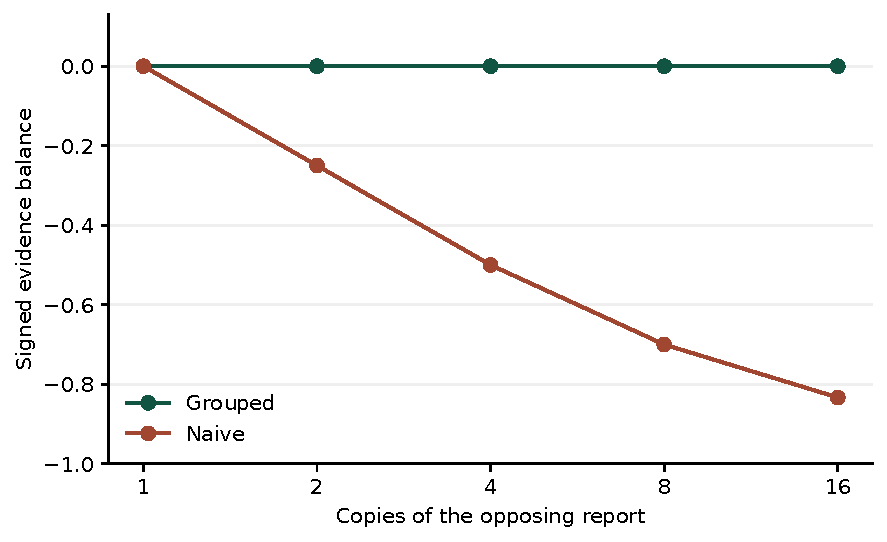
\includegraphics[width=.72\linewidth]{duplicate-injection.pdf}
\caption{One supporting observation competes with an opposing observation repeated across documents. All documents are retained in this experiment.}
\end{figure}
On the synthetic test set, grouped voting matched 300/360 expected evidence verdicts. Removing grouping or temporal filtering separately reduced this to 270/360. Ignoring contradictory evidence reduced it to 180/360. Fixed-budget search and removing the final offset check yielded the same verdict accuracy as the full configuration. All 30 multilingual and all 30 two-hop instances were missed by the default rule pipeline. For 150 decisive test responses with known simulator truth, the calibration Brier score was .150. Repeated templates make this estimate unsuitable for deployment confidence.

The first neural diagnostic returned 24 decisive verdicts, including 10 correct ones, and matched two of 39 citations to an annotated rationale with the predicted stance. On the next 80 claims the ungated variant produced 53 decisive answers and 32 correct overall verdicts. The learned gate produced 18 decisive answers and 38 correct overall verdicts, including 11 correct decisive answers. Citation precision against annotated rationales was 6/19. The Wilson 95\% interval for decisive answer accuracy was $[.386,.797]$. Citation annotations may omit other defensible passages, and multiple citations for one query are dependent. These results do not justify general-purpose scientific verification.

The neural gated run used roughly 1.36 GiB peak resident memory. Index construction and warm-up took about 133 seconds; median and 95th-percentile query latencies were about 0.45 and 0.57 seconds in the recorded run. The repository retains per-query measurements. The extractive BM25 baseline selected an annotated rationale on 44/300 claims; pure latent retrieval did so on 17/300. An extra local search for independent verbatim corroboration emitted no answers and used 600 retrievals on the same 300 claims. It is a limited search-and-check proxy for one aspect of SAFE.

\section{Failure analysis and implications}
Duplicating an opposing report sixteen times could hide the primary record from even a ten-document budget. The grouping stage then saw a single family with no competing stance. This provides a counterexample to an unconditional duplication guarantee. Independent verification of publisher identity, quote lineage and validity metadata remains necessary. Missing metadata can cause unnecessary abstention. English NLI errors, restricted question forms and the absence of a real-world provenance test set limit generality. Synthetic report attribution must never be used to accuse a real author of copying. Users should treat decisions as claims about the indexed evidence.

\section{Reproducibility and conclusion}
The repository includes the SDK, CLI, service, browser interface, synthetic generator, fit scripts, checkpoints, constrained dependency versions, data hashes and raw results. Experiments require no paid APIs. Public artifacts identify external dataset terms and model revisions. A replication with independently annotated source relationships, document versions and open-web retrieval would test the main unresolved interaction between evidence availability and aggregation. This technical report has no journal or conference acceptance claim. The evaluation question is closest to empirical information retrieval and evidence-grounded NLP as studied at SIGIR, ACL and EMNLP.
\bibliographystyle{plain}
\bibliography{../research/references}
\end{document}
